\subsection{Recobrimento 1-conexo quando X slsc} %afirmação aqui significa teorema/proposição/colorário/lema
\label{recobrimento-1-conexo-prop}
\begin{titlemize}{Lista de dependências}
    \item \hyperref[espaco-de-recobrimento-def]{Espaço de recobrimento};\\
	\item \hyperref[espaço-semi-localmente-simplesmente-conexo-def]{Espaço semi-localmente simplesmente conexo};\\ %'dependencia1' é o label onde o conceito Dependência 1 aparece (--à arrumar um padrão para referencias e labels--) 
	\item \hyperref[espaço-1-conexo-def]{Espaço 1-conexo};\\
    \item \hyperref[levantamento-de-homotopia-prop]{Levantamento de homotopia};\\
% quantas dependências forem necessárias.
\end{titlemize}

\begin{thm}[Recobrimento 1-conexo]% ou af(afirmação)/prop(proposição)/corol(corolário)/lemma(lema)/outros ambientes devem ser definidos no preambulo de Alg.Top-Wiki.tex 
	Seja $X$ um espaço conexo por caminhos e localmente conexo por caminhos. Então $X$ admite um recobrimento 1-conexo $p:E\rightarrow X$ se e somente se $X$ for semi-localmente simplesmente conexo.\\
\end{thm}
\begin{dem}
    Por um lado, se $X$ admite um recobrimento 1-conexo $p:E\rightarrow X$, isto é, com $E$ 1-conexo, temos a seguinte situação:\newline

    Sabemos que, por definição de recobrimento, para todo $x\in X$ existe $U\subset X$ vizinhança de $x$ que é uniformemente recoberto, conforme terminologia apresentada em \ref{espaco-de-recobrimento-def}.

    Assim, mostremos que, dada a inclusão $i:U\rightarrow X$, temos que $i_*:\pi(U,x)\rightarrow \pi(X,x)$ é um mapa trivial.

    Tome $[\alpha]_U \in \pi_1(U,x)$ qualquer. Denotemos $i_*([\alpha]_U)=[i\circ \alpha]$ por $[\alpha]\in \pi(X,x)$.

    Fixado $e\in E$ tal que $p(e)=x$, é possível levantar a curva $\alpha$ para $\tilde{\alpha}_e\in \Omega (E,e)$ nos termos de \ref{levantamento-de-caminhos-prop}. Assim, $\tilde{\alpha}_e$ é  curva com início em $e$. Considerando que $\alpha$ é fechada, temos que $\tilde{\alpha}_e(1)=e=c_e(1)$, onde $c_e$ é a curva constante em $e$.

    Como $E$ é 1-conexo, é possível aplicar o corolário 4 de \ref{levantamento-de-homotopia-prop}, que é aplicação direta da definição de 1-conexo, e concluir que $\tilde{\alpha}_e$ e $c_e$ são homotópicos por uma homotopia relativa a $\partial I$.
    
    Assim, $c_x$ curva constante parada no mesmo $x$ anterior em $X$, pode ser levantada a $c_e$ em $E$, enquanto $\alpha$ pode ser levantado a $\tilde{\alpha}_e$, e os levantamentos destas duas curvas são homotópicos relativamente a $\partial I$. Nesta situação, é possível aplicar o corolário 3 também de \ref{levantamento-de-homotopia-prop}, e concluir que $\alpha$ e $c_x$ são caminhos homotópicos relativamente a $\partial I$.

    Em outras palavras, $i_*[\alpha]_U=[\alpha]=[c_x]$. O que implica que $i_*$ de fato envia sempre na mesma classe e é mapa trivial.\newline\newline




    Na outra implicação, temos que se $X$ é semi-localmente simplesmente conexo:\newline
    
    A proposição \ref{recobrimento-1-conexo-em-bijecao-com-P(X,x)} é um indício de que o espaço $P(X,x_0)$ ali definido pode ser um bom candidato a espaço 1-conexo.

    De fato, iremos realizar esta verificação. 

    Lembre que $P(X,x_0)$ é definido por $\{[\gamma]| ~\gamma:I\rightarrow X\text{ ~ }\gamma(0)=x_0\}$, isto é, o espaço das classes relativas a $\partial I$ dos caminhos em $X$ que começam em $x_0$.

    Considere a projeção $q: P(X,x_0)\rightarrow X$ definida por 

    $$q([\gamma])=\gamma(1)$$

    Esta é uma função \textbf{bem definida} porque se duas curvas $\gamma_1$ e $\gamma_2$ estão na mesma classe de $P(X,x_0)$, isso significa que existe homotopia entre elas que fixa seus pontos extremos e, de fato, $q([\gamma_1])=\gamma_1(1)=\gamma_2(1)=q([\gamma_2])$.

    Além disso, $q$ é um mapa \textbf{sobrejetor} porque se $X$ é conexo por caminhos, existem curvas $\gamma$ que ligam $x_0$ a qualquer outro ponto $x\in X$. De fato, $\gamma(1)$ pode ser qualquer ponto de $X$ variando a curva.

    Considere o seguinte espaço:

    $$\mathcal{B}=\{U\subset X | U \text{ é aberto conexo por caminhos e } i^*:\pi_1(U)\rightarrow \pi_1(X)\text{ é trivial }\}$$

    Note que $i^*$ é trivial para toda escolha de ponto base em $U$, uma vez que esse aberto é conexo por caminhos. Por isso, foi escrito $\pi_1(U)$ e  $\pi_1(X)$ ao invés de  $\pi_1(U,x)$ e  $\pi_1(X,x)$ para algum $x\in U$.

    Verifiquemos que esta é uma \textbf{base para a topologia de $X$}

     Por $X$ ser semi-localmente simplesmente conexo, para todo $x\in X$ existe aberto $U$ vizinhança de $x$ tal que $i^*:\pi_1(U,x)\rightarrow \pi_1(X,x)$ é trivial. Como, além disso, $X$ é localmente conexo por caminhos, sabemos que existe $V\subset U$ conexo por caminhos que também é vizinhança de $x$. Assim, a composição dos homomorfismos induzidos por inclusões $\pi_1(V,x)\rightarrow \pi_1(U,x)\rightarrow \pi_1(X,x)$ também deve ser trivial. Dessa forma, existe $V\in \mathcal{B}$ que é vizinhança de $x$. Este argumento mostra que os abertos de $\mathcal{B}$ cobrem $X$.

     Além disso, a intersecção de quaisquer dois abertos em $\mathcal{B}$ é novamente um aberto em $\mathcal{B}$ pois a intersecção de dois abertos conexos por caminhos é um aberto conexo por caminhos. Ele será subespaço dos dois abertos iniciais e será possível construir uma composição como a do parágrafo anterior para mostrar que o homomorfismo induzido entre os grupos fundamentais da intersecção e de $X$ é trivial.

     Agora, dado um aberto $U\in \mathcal{B}$ e um caminho $\gamma:I\rightarrow X$ com $\gamma(0)=x_0$ e $\gamma(1)=x\in U$, defina por

     $$U_{[\gamma]}=\{[\gamma* \eta]\in P(X,x_0)| \eta:I\rightarrow U\text{ tal que } \eta(0)=\gamma(1)\}$$


     um aberto de $P(X,x_0)$. Note que $U_{[\gamma]}$ depende apenas da classe $\gamma$.

     Tome duas curvas quaisquer $\gamma$ e $\gamma'$ com início em $x_0$ e que terminam em algum ponto de $U\in \mathcal{B}$, como acima. Os abertos $U_{[\gamma]}$ e $U_{[\gamma']}$ são iguais se e somente se $[\gamma']\in U_{[\gamma]}$.
     
     De fato, se $U_{[\gamma]}=U_{[\gamma']}$ temos que $$[\gamma']=[\gamma'*c_{\gamma'(1)}]\in U_{[\gamma']}=U_{[\gamma]}.$$ Por outro lado, se $[\gamma']\in U_{[\gamma]}$, então $\gamma'\sim \gamma *\eta ~(\text{rel }\partial I)$ para algum $\eta$ em $U$ com início em $\gamma(1)$, o que significa que todo elemento $\varepsilon\in U_{[\gamma']}$ é tal que $$\varepsilon\sim\gamma'*\mu\sim (\gamma*\eta)*\mu (\text{rel }\partial I)$$ para algum $\mu$ em $U$ com início em $\gamma'(1)$. Isso indica que $[\varepsilon]\in U_{[\gamma]}$ e $U_{[\gamma']}\subset U_{[\gamma]}$. Além disso, todo elemento $[\epsilon] \in U_{[\gamma]}$ é tal que $$\epsilon \sim \gamma * \mu' \sim \gamma*\eta*\overline{\eta}*\mu'\sim \gamma' *\overline{\eta}*\mu'(\text{rel }\partial I)$$ e, portanto, $[\epsilon]\in U_{[\gamma']}$. Observe a situação aqui descrita na imagem \ref{fig:cobertura-P(X,x_0)} a seguir.

     \begin{figure}[h!]
         \centering
         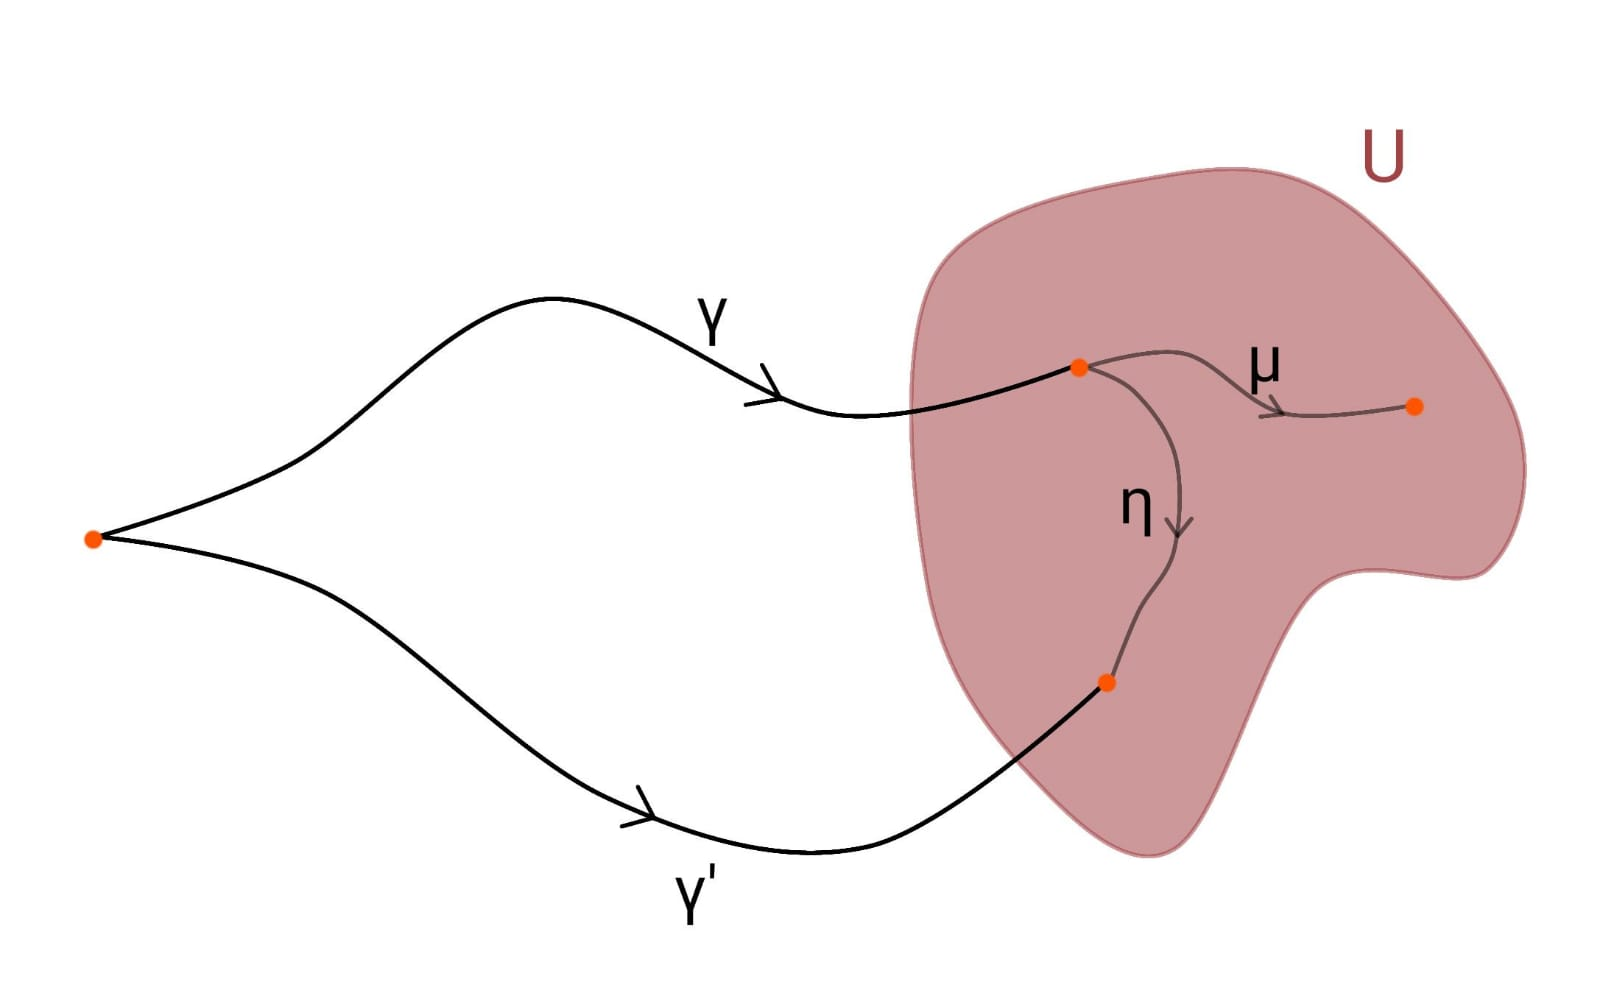
\includegraphics[width=0.8\linewidth]{conteudo/fig-cobertura-P(X,x_0).jpeg}
         \caption{Verificação de quando dois abertos $U_{[\gamma]}$ são iguais}
         \label{fig:cobertura-P(X,x_0)}
     \end{figure} 

     
     Verifiquemos que abertos desta forma constituem uma base para $P(X,x_0)$ e, além disso, que $q:U_{[\gamma]}\rightarrow U$ é um homeomorfismo, o que nos aproxima da verificação de que $q:P(X,x_0)\rightarrow X$ é um espaço de recobrimento.\newline

     De fato, temos as seguintes informações:

     \begin{enumerate}
        \item  $q:U_{[\gamma]}\rightarrow U$ é mapa injetor.\newline
        
        Escolhas diferentes de $\eta$ em $U$ que ligam $\gamma(1)$ a um mesmo ponto $x\in U$, isto é, dois caminhos $\eta_1$ e $\eta_2$ nessas condições tais que $q([\gamma*\eta_1])=q([\gamma*\eta_2])$, são tais que $\eta_1\sim \eta_2 (\text{rel }\partial I)$. Isso ocorre porque $i^*:\pi_1(U,x)\rightarrow \pi_1(X,x)$ é trivial, o que leva a conclusão de que dada a curva fechada $\eta_1* \overline{\eta_2}$ com ponto base $x$, temos a igualdade $[\eta_1* \overline{\eta_2}]=[c_x]\in \pi_1(X,x)$ e, portanto, $$\eta_1\sim\eta_1*(\overline{\eta_2}*\eta^2)\sim (\eta_1*\overline{\eta_2})*\eta^2\sim c_x*\eta_2\sim  \eta_2~(\text{rel }\partial I).$$  Dessa forma, $\gamma*\eta_1\sim \gamma*\eta_2 (\text{rel }\partial I)$ e, portanto, $[\gamma*\eta_1]=[\gamma*\eta_2]$. A situação é descrita na figura \ref{fig:restricao-de-q-é-injetor}.

        \begin{figure}[h!]
         \centering
         \includegraphics[width=0.8\linewidth]{conteudo/fig-restricao-de-q-é-injetor.jpeg}
         \caption{Restrição de $q$ a $U_{[\gamma]}$ é mapa injetor}
         \label{fig:restricao-de-q-é-injetor}
     \end{figure} 
     
         \item $q:U_{[\gamma]}\rightarrow U$ é mapa sobrejetor.\newline
         
         Como $U$ é conexo por caminhos, sempre é possível encontrar curva $\eta$ em $U$ que ligue $\gamma(1)$ a qualquer outro ponto de $U$.\newline
         
         \item $\tilde{\mathcal{B}}=\{U_{[\gamma]}|~U\in \mathcal{B}, \gamma:I\rightarrow X\text{ com }\gamma(0)=x_0\text{ e }\gamma(1)=x\in U\}$ é base para a topologia de $P(X,x_0)$.\newline
         
        Os abertos de $\tilde{\mathcal{B}}$ realmente cobrem $P(X,x_0)$ porque dado qualquer $[\gamma]\in P(X,x_0)$, se $\gamma(1)=x$, então existe $U\in \mathcal{B}$ vizinhança de $x$ de forma que $[\gamma]\in U_{[\gamma]}$.
        Além disso, dados $U_{[\gamma_1]} $ e $V_{\gamma_2}$ quaisquer em $\tilde{\mathcal{B}}$ e um elemento $[\gamma]\in U_{\gamma_1}\cap V_{\gamma_2}$, temos que $U_{[\gamma]}= U_{[\gamma_1]}$ e $V_{[\gamma]}=V_{[\gamma_2]}$, pois mostramos anteriormente que em geral $U_{[\gamma]}=U_{[\gamma']}$ se e somente se $[\gamma']\in U_{[\gamma]}$. Assim, $\gamma(1)\in U$, $\gamma(1)\in V$ e é possível tomar $W\in \mathcal{B}$ tal que $W\subset U\cap V$ é vizinhança de $\gamma(1)$, uma vez que $\mathcal{B}$ é base. Dessa forma, $W_{[\gamma]}\subset U_{[\gamma]}\cap V_{[\gamma]}=U_{[\gamma_1]}\cap V_{[\gamma_2]}$ pertence a $\tilde{\mathcal{B}}$ e contém $[\gamma]=[\gamma*c_{\gamma(1)}]$\newline
         

         \item $q:U_{[\gamma]}\rightarrow U$ é de fato homeomorfismo.\newline
         
            Seja $V\subset U$ aberto em $\mathcal{B}$. A pré-imagem desse aberto pela restrição de $q$ em $U_[\gamma]$ é $q^{-1}(V)\cap U_{[\gamma]}= V_{[\gamma']}$ para qualquer $[\gamma']\in U_{[\gamma]}$ tal que $\gamma'(1)\in V$, uma vez que $V_{[\gamma']} \subset U_{[\gamma']}=U_{[\gamma]}$ e já vimos que $q:V_{[\gamma']}\rightarrow V$ é uma bijeção. 
            
            De fato, se $V'\subset U$ é aberto qualquer, $V'=\underset{\lambda\in \Lambda, U_\lambda\in \mathcal{B}}{\bigcup} U_\lambda$ união enumerável de abertos e a pré imagem de $V'$ pela restrição de $q$ em $U_{[\gamma]}$ é $$q^{-1}(V')\cap U_{[\gamma]} =\underset{\lambda\in \Lambda, U_\lambda\in \mathcal{B}}{\bigcup} q^{-1}(U_\lambda)\cap U_{[\gamma]} = \underset{\lambda\in \Lambda, U_\lambda\in \mathcal{B}}{\bigcup} (U_\lambda)_{[\gamma_\lambda]}$$ para qualquer $[\gamma_\lambda]\in U_{[\gamma]}$ tal que $\gamma_\lambda(1)\in U_\lambda$. De fato, a pré-imagem é união enumerável de abertos e, portanto, aberta.
            
            
            Além disso, como $q(V_{[\gamma]})=V$ aberto e $\tilde{\mathcal{U}}$ é base, temos que dado qualquer aberto $V''\subset U_{[\gamma]}$ é $V''=\underset{\lambda \in \Lambda, U_\lambda \in \tilde{\mathcal{U}}}{\bigcup} U_\lambda$ união enumerável de abertos e então $q(V'')=\underset{\lambda \in \Lambda, U_\lambda \in \tilde{\mathcal{U}}}{\bigcup} q(U_\lambda)$, onde $q(U_\lambda)\in \mathcal{B}$ para todo $\lambda \in \Lambda$. Isto é, $q(V'')$ é união enumerável de abertos e, portanto, aberto.\newline

        \item $q:P(X,x_0)\rightarrow X$ é contínuo.\newline
        
            Para todo aberto $V\subset X$, temos que $V=\underset{\lambda\in \Lambda, V_\lambda \in \mathcal{B}}{\bigcup} V_\lambda$ para certos abertos $V_\lambda$ em $\mathcal{B}$.

            Temos que $$q^{-1}(V)=q^{-1}(\underset{\lambda\in \Lambda, V_\lambda \in \mathcal{B}}{\bigcup} V_\lambda)=\underset{\lambda\in \Lambda, V_\lambda \in \mathcal{B}}{\bigcup}q^{-1}(V_\lambda),$$ onde $q^{-1}(V_\lambda)=\underset{\gamma, (V_\lambda)_[\gamma] \in \tilde{\mathcal{B}}}{\bigcup} (V_\lambda)_{[\gamma]}$.

            Assim, todo $[\gamma]\in q^{-1}(V)$ é tal que $\gamma(1)\in V$ e, portanto, $\gamma(1)\in V_{\lambda_0}$ para algum $\lambda_0\in \Lambda$. Isto significa que $[\gamma]\in (V_{\lambda_0})_\gamma\subset q^{-1}(V)$ aberto. Portanto, $q^{-1}(V)$ é de fato aberto, como queríamos.\newline\newline
     \end{enumerate}


    Assim, temos que para todo $x\in X$ existe $U\in \mathcal{B}$ vizinhança de $x$ tal que  $p^{-1}(U)=\underset{[\gamma]}{\sqcup} U_{[\gamma]}$, onde cada $U_{[\gamma]}$ é homeomorfo a $U$. Essa união é disjunta pois se $U_{[\gamma_1]}\neq U_{[\gamma_2]}$ e $[\gamma]\in U_{[\gamma_1]}\cap U_{[\gamma_2]}$, então $U_{[\gamma]}=U_{[\gamma_1]}$ e $U_{[\gamma]}=U_{[\gamma_2]}$, o que implica $U_{[\gamma_1]}=U_{[\gamma_2]}$, uma contradição. Portanto, $U$ é aberto uniformemente recoberto de $X$ e isso conclui a nossa demonstração de que $P(X,x_0)$ é espaço de recobrimento.\newline

    Resta, por último, verificar que $P(X,x_0)$ é 1-conexo:

    \begin{enumerate}
        \item $P(X,x_0)$ é conexo por caminhos.\newline
        
            De fato, para todo $[\gamma]\in P(X,x_0)$, tome $\gamma_t:[0,1]\rightarrow X$ como a curva definida por 

            $$\begin{cases}
                \gamma(s), \text{ se }s\in [0,t]\\
                \gamma(t), \text{ se }s\in [t,1]
            \end{cases}$$

            Assim a curva $t\mapsto [\gamma_t]$ é um caminho em $P(X,x_0)$ que começa em $[c_{\gamma(0)}]=[c_{x_0}]$, curva constante em $\gamma(0)=x_0$, e termina em $[\gamma]$.

            Como isso vale para todo $[\gamma]$ em $P(X, x_0)$, então esse espaço é conexo por caminhos.\newline
        
        \item $\pi_1(P(X,x_0), [c_{x_0}])=0$\newline
        
            Para esta verificação mostraremos que $p_*: \pi_1(P(X,x_0), [c_{x_0}])\rightarrow \pi_1(X,x_0)$ é trivial.\newline

            Um elemento na imagem de $p_*$ é da forma $[\gamma]$ onde $\gamma$ é curva fechada com ponto base $x_0$ e seu levantamento também deve ser curva fechada, neste caso com ponto base $[c_{x_0}]$. Foi visto no item anterior que $t\mapsto [\gamma_t]$ levanta $\gamma$, começando em $[x_0]$ e terminando em $[\gamma_1]=[\gamma]$. Se esse levantamento é uma curva fechada, então $[\gamma]=[c_{x_0}]$ e o mapa de fato é trivial.

            Como $p_*$ é injetivo segundo o lema \ref{homomorfismo-induzido-por-recobrimento-prop}, então o fato de ser trivial implica $\pi_1(P(X,x_0), [c_{x_0}])=0$, como queríamos.\newline
        
    \end{enumerate}

    Assim, verificamos que $q: P(X,x_0)\rightarrow X$ é de fato um recobrimento 1-conexo e concluí-se por fim que, nas condições do enunciado, quando $X$ é semi-localmente simplesmente conexo, $X$ admite recobrimento 1-conexo.
    
\end{dem}

\begin{titlemize}{Lista de consequências}
	\item \hyperref[pertence-a-base-se-e-somente-se-possui-i-trivial]{Proposição - nova descrição da base $\mathcal{B}$};\\ %'consequencia1' é o label onde o conceito Consequência 1 aparece
    %\item \hyperref[espaço-1-conexo-def]{Espaço 1-conexo}
\end{titlemize}
